\documentclass[tikz,border=3pt]{standalone}
\usepackage[utf8]{inputenc}
\usepackage[T1]{fontenc}
\usepackage{lmodern}
\renewcommand{\familydefault}{\sfdefault}
\usepackage{amsmath}
\usepackage{sansmath}\sansmath
\usepackage{pgfplots}\pgfplotsset{compat=1.18,/pgf/number format/use comma,/pgf/number format/1000 sep={.}}
\usetikzlibrary{arrows.meta,calc,positioning,decorations.pathmorphing,patterns}
% paleta del sitio
\definecolor{nar}{HTML}{E8680C}\definecolor{narc}{HTML}{FFB35C}\definecolor{hielo}{HTML}{FFF3E8}
\definecolor{tinta}{HTML}{1D1D1F}\definecolor{gris}{HTML}{6E6E73}\definecolor{lila}{HTML}{7C5CF0}
\definecolor{azul}{HTML}{2F6FD6}\definecolor{menta}{HTML}{17A673}\definecolor{coral}{HTML}{E8342A}
\pgfplotsset{base/.style={axis lines=left,grid=major,grid style={gris!20},tick label style={font=\small},label style={font=\small},axis line style={tinta!80}}}
\begin{document}
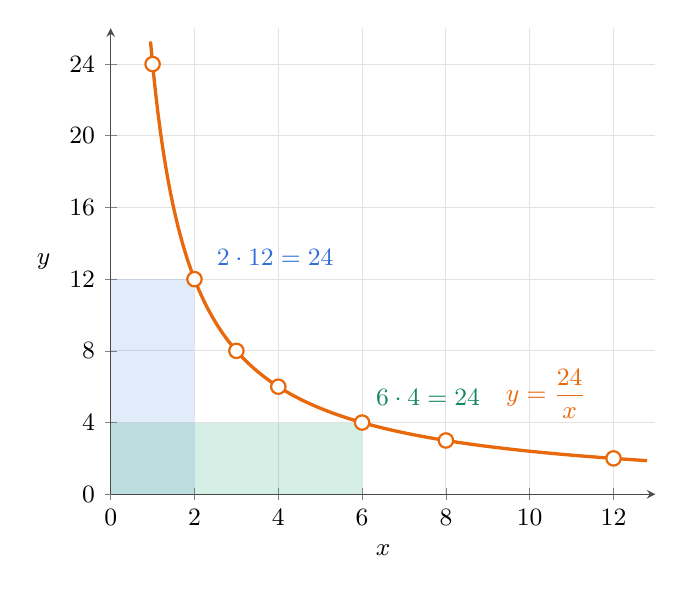
\begin{tikzpicture}
\begin{axis}[base,width=8.5cm,height=7.5cm,xmin=0,xmax=13,ymin=0,ymax=26,xtick={0,2,...,12},ytick={0,4,...,24},xlabel={$x$},ylabel={$y$},ylabel style={rotate=-90},clip=false]
\fill[azul,fill opacity=.14] (axis cs:0,0) rectangle (axis cs:2,12);
\fill[menta,fill opacity=.18] (axis cs:0,0) rectangle (axis cs:6,4);
\addplot[nar,very thick,domain=0.95:12.8,samples=200] {24/x};
\addplot[only marks,mark=*,mark options={fill=white,draw=nar,thick},mark size=2.6pt] coordinates {(1,24)(2,12)(3,8)(4,6)(6,4)(8,3)(12,2)};
\node[azul,font=\small\bfseries,anchor=west] at (axis cs:2.3,13.2) {$2 \cdot 12 = 24$};
\node[menta!80!black,font=\small\bfseries,anchor=south west] at (axis cs:6.1,4.4) {$6 \cdot 4 = 24$};
\node[nar,font=\small\bfseries,anchor=west] at (axis cs:9.2,5.6) {$y = \dfrac{24}{x}$};
\end{axis}
\end{tikzpicture}
\end{document}
